\documentclass[tikz,border=4pt]{standalone}
\usepackage{tikz}
\usetikzlibrary{arrows.meta, positioning, shapes.geometric, fit, backgrounds}

\begin{document}
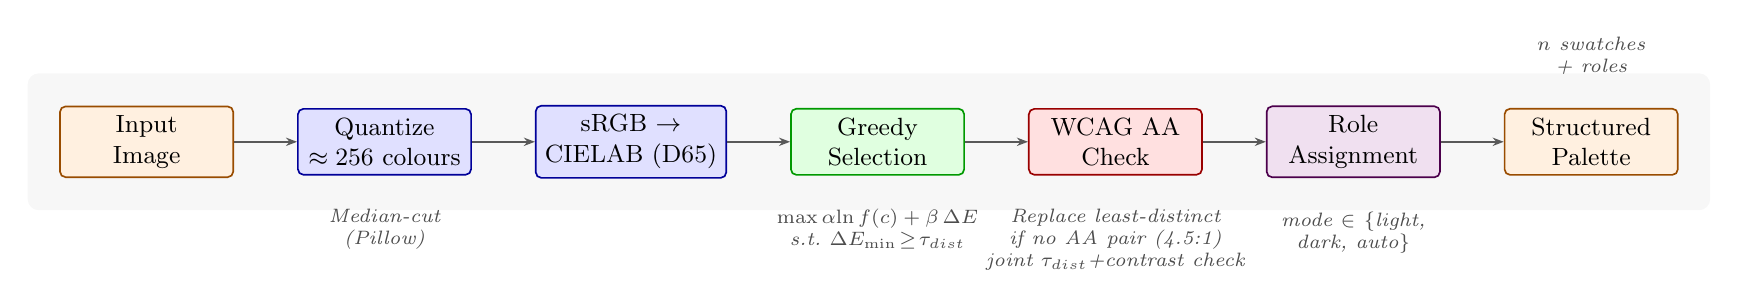
\begin{tikzpicture}[
  node distance = 5mm and 8mm,
  every node/.style = {font=\small},
  box/.style = {
    draw, rounded corners=2pt, minimum height=8mm, minimum width=22mm,
    text centered, align=center, fill=#1!12, draw=#1!60!black, line width=0.6pt
  },
  box/.default = blue,
  arrow/.style = {-{Stealth[length=4pt]}, line width=0.7pt, gray!70!black},
  note/.style = {font=\scriptsize\itshape, text=gray!60!black, align=center},
]

% ── main pipeline nodes ────────────────────────────────────────────
\node[box=orange] (img)  {Input\\Image};

\node[box=blue,   right=of img]   (quant) {Quantize\\$\approx256$ colours};

\node[box=blue,   right=of quant] (lab)   {sRGB $\to$\\CIELAB (D65)};

\node[box=green,  right=of lab]   (greedy){Greedy\\Selection};

\node[box=red,    right=of greedy](wcag)  {WCAG AA\\Check};

\node[box=violet, right=of wcag]  (roles) {Role\\Assignment};

\node[box=orange, right=of roles] (out)   {Structured\\Palette};

% ── arrows ─────────────────────────────────────────────────────────
\foreach \a/\b in {img/quant, quant/lab, lab/greedy, greedy/wcag,
                   wcag/roles, roles/out}
  \draw[arrow] (\a) -- (\b);

% ── annotation notes ───────────────────────────────────────────────
\node[note, below=3mm of quant] {Median-cut\\(Pillow)};

\node[note, below=3mm of greedy] {$\max \alpha\!\ln f(c) + \beta\,\Delta E$\\
  s.t.\ $\Delta E_{\min} \!\geq\! \tau_{\text{dist}}$};

\node[note, below=3mm of wcag] {Replace least-distinct\\
  if no AA pair (4.5:1)\\
  \textit{joint $\tau_{\text{dist}}$+contrast check}};

\node[note, below=3mm of roles] {mode $\in$ \{light,\\dark, auto\}};

% ── output swatches (decorative) ──────────────────────────────────
\node[note, above=3mm of out, xshift=0pt] {$n$ swatches\\+ roles};

% ── background panel ──────────────────────────────────────────────
\begin{scope}[on background layer]
  \node[fill=gray!6, rounded corners=4pt, inner sep=4mm,
        fit=(img)(out)(quant)(lab)(greedy)(wcag)(roles)] {};
\end{scope}

\end{tikzpicture}
\end{document}
